\begin{figure}[!htb]
\begin{center}
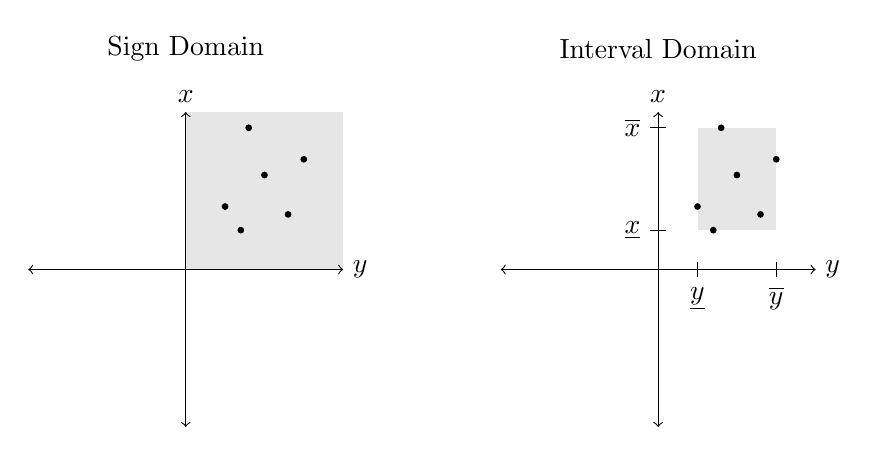
\begin{tikzpicture}
 		\coordinate (A) at (-1,-2);
		\coordinate (B) at (-1,2);
		\coordinate (C) at (-3,0);
		\coordinate (D) at (1,0);
		
		\draw [draw=none, fill=gray, fill opacity=0.2] (-1,0) -- (-1,2) -- (1,2) -- (1,0) -- cycle;
		
		%Axis
		\draw[<->] (A) -- (B) node [above] {$x$};
		\draw[<->] (C) -- (D) node [right] {$y$};
		
		
		\filldraw[black] (-0.5,0.8) circle (1pt);	
		\filldraw[black] (0,1.2) circle (1pt);
		\filldraw[black] (0.5,1.4) circle (1pt);	
		\filldraw[black] (-0.2,1.8) circle (1pt);
		\filldraw[black] (-0.3,0.5) circle (1pt);	
		\filldraw[black] (0.3,0.7) circle (1pt);	
		
		
		\node at (-1,2.8) {Sign Domain};
		
		\coordinate (E) at (5,-2);
		\coordinate (F) at (5,2);
		\coordinate (G) at (3,0);
		\coordinate (H) at (7,0);
		
		\draw [draw=none, fill=gray, fill opacity=0.2] (5.5,0.5) -- (5.5,1.8) -- (6.5,1.8) -- (6.5,0.5) -- cycle;
		
		\draw[-] (5.5,0.1) -- (5.5,-0.1);
		\draw[-] (6.5,0.1) -- (6.5,-0.1);
		
		\draw[-] (4.9,1.8) -- (5.1,1.8);
		\draw[-] (4.9,0.5) -- (5.1,0.5);
		
		\node at (5,1.8)[left, xshift=-1mm] {$\overline{x}$};
		\node at (5,0.5)[left, xshift=-1mm] {$\underline{x}$};
		
		\node at (5.5,0)[below, yshift=-1mm] {$\underline{y}$};
		\node at (6.5,0)[below, yshift=-1mm] {$\overline{y}$};
		
		%Axis
		\draw[<->] (E) -- (F) node [above] {$x$};
		\draw[<->] (G) -- (H) node [right] {$y$};
		
		\filldraw[black] (5.5,0.8) circle (1pt);	
		\filldraw[black] (6,1.2) circle (1pt);
		\filldraw[black] (6.5,1.4) circle (1pt);	
		\filldraw[black] (5.8,1.8) circle (1pt);
		\filldraw[black] (5.7,0.5) circle (1pt);	
		\filldraw[black] (6.3,0.7) circle (1pt);		
		
		\node at (5,2.8) {Interval Domain};		
		
		
\end{tikzpicture}
\end{center}
\caption{A diagram comparing abstract representation for a set of states. In this example a concrete state consists only of two scalar variable values $x$ and $y$. Therefore a concrete state can be represented as a point in the plane. The sign domain state, which is abstracting the marked concrete states, spans an entire quadrant of the coordinate system, whereas the interval domain state only occupies the rectangle encasing the states.}\label{fig:domaincomparison}
\end{figure}
